%\title{גיאומטריה חישובית}
\documentclass{article}
\usepackage{graphicx}
\usepackage[utf8x]{inputenc}
\usepackage[english,hebrew]{babel}
\selectlanguage{hebrew}
\usepackage[normalem]{ulem}
\usepackage[top=2cm,bottom=2cm,left=2.5cm,right=2cm]{geometry}
\usepackage[fleqn]{amsmath}
\usepackage{mathtools}
\usepackage{amsfonts, amsthm, amssymb, amsmath, cancel, enumitem, comment}
\DeclarePairedDelimiter\ceil{\lceil}{\rceil}
\DeclarePairedDelimiter\floor{\lfloor}{\rfloor}
\newenvironment{spmatrix}[1]
 {\def\mysubscript{#1}\mathop\bgroup\begin{pmatrix}}
 {\end{pmatrix}\egroup_{\textstyle\mathstrut\mysubscript}}
 
\usepackage{accents}

\newcommand{\uwidehat}[1]{%
  \mathpalette\douwidehat{#1}%
}

\newcommand{\uhat}{\underaccent{\check}}

\makeatletter
\newcommand{\douwidehat}[2]{%
  \sbox0{$\m@th#1\widehat{\hphantom{#2}}$}%
  \sbox2{$\m@th#1x$}
  \sbox4{$\m@th#1#2$}
  \dimen0=\ht0
  \advance\dimen0 -.8\ht2
  \dimen2=\dp4
  \rlap{%
    \raisebox{\dimexpr\dimen0-\dimen2}{%
      \scalebox{1}[-1]{\box0}%
    }%
  }%
  {#2}%
}
\makeatother

\usepackage{titlesec, url, color}

\setcounter{secnumdepth}{4}
\def\titlefootnote{\ifx\protect\@typeset@protect\expandafter\footnote\else\expandafter\@gobble\fi}
\makeatletter
\def\@xfootnote[#1]{\protected@xdef\@thefnmark{#1}\@footnotemark\@footnotetext}

\makeatletter
\titleformat{\paragraph}
{\normalfont\normalsize\bfseries}{\theparagraph}{1em}{}
\titlespacing*{\paragraph}
{0pt}{3.25ex plus 1ex minus .2ex}{1.5ex plus .2ex}

\setcounter{secnumdepth}{5}

\titleformat{\subparagraph}
{\normalfont\normalsize\bfseries}{\thesubparagraph}{1em}{}
\titlespacing*{\subparagraph}
{0pt}{3.25ex plus 1ex minus .2ex}{1.5ex plus .2ex}


\makeatletter
\newcommand*{\saved@uline}{}
\let\saved@uline\uline

\newcommand*{\mathuline}{%
  \mathpalette{\math@uline\saved@uline}%
}
\newcommand*{\math@uline}[3]{%
  % #1: ulem command
  % #2: math style
  % #3: contents
  \mbox{#1{$#2#3\m@th$}}%
}

% optional
\renewcommand*{\uline}{%
  \relax  
  \ifmmode
    \expandafter\mathuline
  \else
    \expandafter\saved@uline
  \fi
}

\newtheorem{theorem}{Theorem}
\newtheorem{claim}{Claim}
\newtheorem{lemma}{Lemma}
\newtheorem{definition}{Definition}
\newtheorem{proposition}{Proposition}
\newtheorem{prob}{Problem}

\title{ גיאומטריה חישובית }
\begin{document}
\maketitle
\section{ סגור קמור}
ניתן לחשוב על הקמור כעל גומייה שנמתחה כך שתקיף את כל הנקודות/ המסמרים, ולאחר מכן שוחררה.\\
\selectlanguage{english}
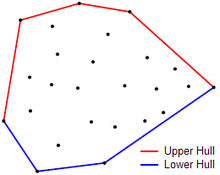
\includegraphics[scale=0.7]{z1.png}
\selectlanguage{hebrew}
\subsection{אלגוריתמים לחישוב סגור קמור}
\subsubsection{אלגוריתם סריקת גרהם}
\begin{itemize}
\item מיין את הנקודות לפי קורדינטות  $x$ כך ש: $x_1 < x_2 < \cdots < x_n$
\item נסרוק את הנקודות משמאל לימין. אחרי $i$ איטרציות, חישבנו את $\hat{CH_i}= \hat{CH}(p_1, \cdots, p_i)$
\end{itemize}
\uline{הבחנה:} לאוסף נקודות $S=\{\ell_1, \cdots, \ell_n \}$ הקמור העליון $\hat{CH}(S)$ הוא אוסף נקודות $Q$ שיוצר שרשרת צלעות עם התכונות הבאות:
\begin{enumerate}
\item $Q_i$ מתחיל ב- $p_1$ ומסתיים ב-$p_i$
\item השרשרת נמצאת מעל כל הנקודות של $S_i$
\item בטיול על שרשרת מ- $p_1$ ל-$p_i$, כל הפניות הן פניות ימינה
\end{enumerate}
מחסנית $\mathcal{S}$ מחזיקה את נקודות הקמור העליון $Q_i$ לפי סדרן.\\ $p_{top}$- הנקודה שנמצאת בראש המחסנית, $p_{2nd}$- הנקודה שנמצאת במחסנית מתחת ל-$p_{top}$\\
\uline{איתחול:} $push(p_1), push(p_2)$\\
\uline{לכל $i$ מ-3 עד $n$ בצע:}
\begin{itemize}
\item 
כל עוד יש במחסנית לפחות 2 נקודות, ושלש הנקודות $p_{2nd}, p_{top}, p_i$ מהוות פניה שמאלה, בצע $pop$
\item בצע $push(p_i)$
\end{itemize}
\uline{טענת נכונות:} לאחר איטרציה $i$, תכולת המחסנית מהווה את $\hat{CH}(S_i)$\\
\uline{סיבוכיות:} $\mathcal{O}(n \log(n))$ )המיון. הערה: כל השאר $\mathcal{O}(n)$(\\
\paragraph{בעיית הגלריה }
למצוא מספר מינימלי של נקודות מהן אפשר לראות את כל המצולע.\\
במצולע קמור מספיקה נקודה אחת.\\
במצולע קעור: ישנן צורות בהן מספיקה נקודה אחת, למשל: \L{star-shaped polygon}\\
\selectlanguage{english}
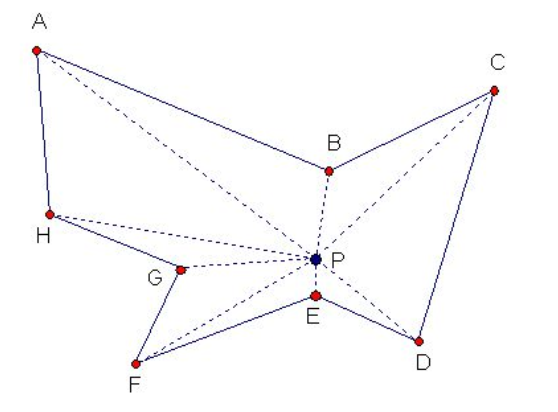
\includegraphics[scale=0.3]{z3.png}
\selectlanguage{hebrew}
\\
אך יתכן שידרשו יותר נקודות:\\
\selectlanguage{english}
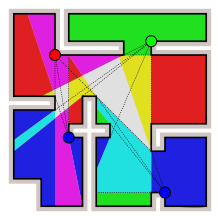
\includegraphics[scale=0.3]{z2.png}
\selectlanguage{hebrew}\\
במצולע דמוי כוכב אפשר לחשב את הסגור הקמור בלי המיון.\\
\textbf{תרגיל:} נניח שאוסף הנקודות $S$ נבחר באקראי בריבוע היחידה. מה ניתן לומר על תוחלת הסיבוכיות של אלגוריתם גרהם?
\subsubsection{אלגוריתם עטיפת המתנות}
\begin{enumerate}
\item מצא את הנקודה הנמוכה ביותר ב-$S$, $p_0$ $(\mathcal{O}(n))$
\item השווה את הנקודות על פי הזווית של $p_0 p_i$ ביחס לקרן ימינה מ-$p_0$, ובחר את $p_1$ בעלת הזווית הקטנה ביותר
\item לכל $i \geq 1:$ לאחר מציאת $p_i$: חפש את $p_{i+1}$ בעלת הזווית הקטנה ביותר בין $\overrightarrow{p_i p_{i+1}}$ לקרן מ-$p_i$ ימינה $(\mathcal{O}(n))$
\end{enumerate}
$\uhat{CH}(S)= <q_1m \cdots, q_h>$\\
$h=|\uhat{CH}(S)|$\\
סיבוכיות כוללת: $\mathcal{O}(n \cdot h)$\\
\uline{שאלה:} מהי תוחלת $|\uhat{CH}(S)|$ כש-$S$ נבחרה באקראי בריבוע היחידה?\\
\uline{תשובה:} $E(h)= \mathcal{O}(\log(n))$\\
\uline{טענה:} $E(|C_{UR}|)= \mathcal{O}(\log(n))$\\
\uline{הגדרה:} הנקודה $p=(x,y)$ שולטת על הנקודה $p'=(x',y')$ אם $x \geq x'$ ו-$y \geq y'$.\\
נקודה ב-$S$ נקראת בלתי נשלטת אם אף נקודה אחרת ב-$S$ לא שולטת עליה.\\
$B$= קבוצת הנקודות הבלתי-נשלטות מ-$S$ ברביע הראשון.\\
$C_{UR} \subseteq B$\\
\uline{טענה:} $E(|B|)= \mathcal{O}(\log(n))$\\
\uline{נימוק:} נמיין את נקודות $S$ בסדר $X$ לא עולה $x_1 \geq \cdots \geq x_n$\\
\uline{הבחנה:}
$p_i=(x_i, y_i)$ לא שלטת אם"ם $y_i$ היא המקסימלית מבין $p_1, \cdots, p_i$ )כלומר, $y_i>y_1, y_2, \cdots, y_{i-1}$(\\
$\Pr(y_i>y_1, y_2, \cdots, y_{i-1})= \frac{1}{i}$\\
$E(|B|)= \sum_{i=1}^n \frac{1}{i}= \mathcal{O}(n)$\\
\textbf{תרגיל:} בהינתן אוסף $S$ של $n$ נקודות, מצא את כל הנקודות הלא נשלטות ב-$S$. )קל: $\mathcal{O}(n^2)$. למצוא יותר יעיל: $\mathcal{O}(n \log(n))$(\\
\subsection{חסם תחתון}
\uline{משפט:} חישוב הסגור הקמור של $n$ נקודות במישור )מוחזר על פי סדר הקודקודים על הסגור( דורש $\Omega(n \log(n))$ פעולות במקרה הגרוע במודל הפעולות האלגבריות.\\
\uline{הוכחה:} נסתמך על כך שמיון דורש $\Omega(n \log(n))$ פעולות במקרה הגרוע.\\
נניח שיש לנו פרוצדורה $A$ לחישוב סגור קמור, נראה אלגוריתם מיון בסיבוכיות $T_A+\mathcal{O}(n)$\\
\textbf{אלגוריתם למיון:}
\uline{קלט:} $x_1, \cdots, x_n$ טבעיים שונים\\
\begin{enumerate}
\item ניצור קלט לבעיית $CH$: $S=\{ p_1=(x_1, x_1^2), c\dots, p_n=(x_n, x_n^2) \}$
\item נפעיל את $A$ ונקבל מצולע $P=CH(S)= <q_1, q_2, \cdots, q_n>$\\
\selectlanguage{english}
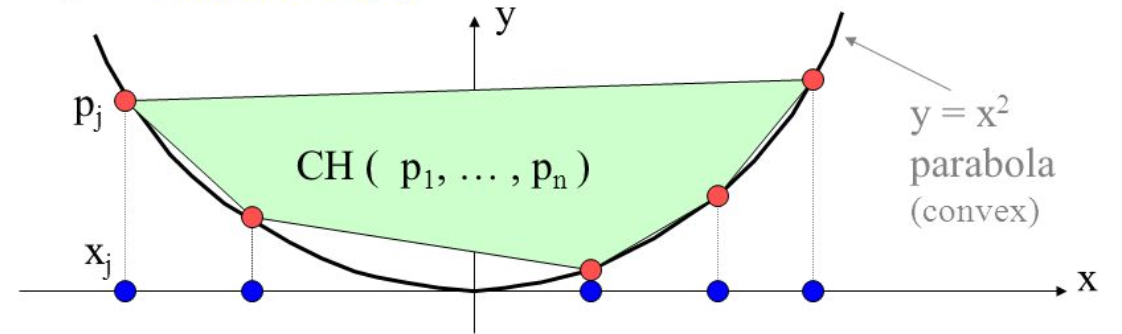
\includegraphics[scale=0.2]{z4.png}
\selectlanguage{hebrew}\\
\item מתוך $P$ נחלץ את הסדרה הממוינת.
\end{enumerate}

\end{document}